\documentclass[twocolumn,10pt]{asme2e}
\special{papersize=8.5in,11in}

\usepackage{graphicx}
\usepackage{amsmath,amssymb}
\usepackage{amsfonts}
\usepackage{url}
\usepackage{nth}
\usepackage[hidelinks]{hyperref}
%\confshortname{IDETC/CIE 2009}
%\conffullname{the ASME 2009 International Design Engineering Technical Conferences \&\\
%	Computers and Information in Engineering Conference}

%%%%% for date in a single month, use
%\confdate{24-28}
%\confmonth{September}
%%%%% for date across two months, use
%\confdate{August 30-September 2}
%\confyear{2009}
%\confcity{San Diego}
%\confcountry{USA}

%%% Replace DETC2009/MESA-12345 with the number supplied to you 
%%% by ASME for your paper.
\papernum{CS289A Course Project}

%%% You need to remove 'DRAFT: ' in the title for the final submitted version.
\title{DRAFT: AN ARTICLE CREATED USING \LaTeX2\raisebox{-.3ex}{$\epsilon$}\ IN ASME FORMAT}

%%% first author
\author{Harry H. Cheng
	\affiliation{
		Integration Engineering Laboratory\\
		Department of Mechanical and Aeronautical Engineering\\
		University of California\\
		Davis, California 95616\\
		Email: hhcheng@ucdavis.edu
	}	
}

%%% second author
%%% remove the following entry for single author papers
%%% add more entries for additional authors
\author{First Coauthor\thanks{Address all correspondence to this author.} \\
	{\tensfb Second Coauthor}     
	\affiliation{Department or Division Name\\
		Company or College Name\\
		City, State (spelled out), Zip Code\\
		Country (only if not U.S.)\\
		Email address (if available)
	}
}

\begin{document}
	
	\maketitle

\maketitle    

%%%%%%%%%%%%%%%%%%%%%%%%%%%%%%%%%%%%%%%%%%%%%%%%%%%%%%%%%%%%%%%%%%%%%%
\begin{abstract}
{\it This article illustrates preparation of ASME paper using \LaTeX2\raisebox{-.3ex}{$\epsilon$}. An abstract for an ASME paper should be less than 150 words and is normally in italics.}
\end{abstract}

\section{Introduction}

\par Macroscopic freeway traffic models are widely used by transportation engineers in order to design controllers and perform re-routing or road management to improve performance of the system; for instance, increasing total traveled distance and decreasing total travel time of vehicles in the network. A crucial component of this process of traffic management is simulation of traffic behavior which is usually accomplished using traditional simulators where system's behavior is predicted by the dynamics assumed to govern evolution of traffic.

The burdensome aspect of traffic prediction is that traffic condition is contingent on too many different parameters. For instance, for a given network, the day for which the simulation is required, plays a significant role as traffic regime on weekends varies from the one on workdays. Furthermore, for a particular day, clearly, vehicular traffic in evening differs from the one at midnight. Thus, a decent traffic prediction must incorporate distinct parameters influencing traffic conditions.

\section{Motivation}

As every watchful motorist driving in California freeways can recognize, there are numerous implemented loop detectors in freeway stretches of California that measure and record traffic metrics. These sensors provide traffic data-centers with huge amount of information that must be taken into account while making predictions. The immense existing data and complexity of traffic behavior as a result of being affected by different continuous and discrete variables, motivated the authors to perform traffic prediction deploying neural network and deep learning methods to come up with a traffic simulation which can possibly perform better than the existing traffic simulators\cite{NNreview}. 
\subsection{Fundamental Diagrams}
In transportation engineering, most of macroscopic freeway traffic models take advantage of the assumption of existence of a \textit{fundamental diagram }for each link in the freeway which maps observed vehicular flow in the link to the corresponding vehicular density \cite{Calibration}. Generally, in order to obtain the fundamental diagram for a given link, vehicular density and flow are recorded for various traffic conditions and a curve is fit into the observed data \cite{cassidy}. In first order freeway traffic models which are widely used in controller design procedure, a piece-wise linear function is fit to the data as shown in figure \ref{fig:fd}. Consideration of a piece-wise linear function implies that flow in a link is restricted to be in three different conditions; \textit{free-flow} region which is the left side of the triangular shape with a positive slope ($v_i$), flow being equal to \textit{capacity}($F_i$) which is the peak point of piece-wise linear function and \textit{congested} region corresponding to the right side of the triangular shape with negative slope ($w_i$).
\subsection{Cell Transmission Model}
The most prevalent first-order freeway model presumed to rule dynamics of freeway and extensively in use is Cell Transmission Model \cite{CTM} in which freeway dynamics are captured by density and flow of each link assuming that the link has a triangular fundamental diagram. In CTM, a freeway is divided into $N$ links and discrete time intervals are considered. For a given link $i$ at time $k$, the state of the link (density) is updated by equation \ref{CTM_update} where $n_i(k)$ is the density of vehicles in section $i$ at time $k$, $f_i(k)$ is the flow leaving section $i$ at time $k$ and  $f_{i-1}(k)$ is the flow entering section $i$ from section $i-1$. 
\begin{equation} \label{CTM_update}
n_i(k+1) = n_i(k) - f_i(k) + f_{i-1}(k)
\end{equation}
As stated already, the assumption is that for each link, fundamental diagram is known; thus, for each link flow is evaluated by equation \ref{flow_equation} where $\bar{n}$ is the jam density or maximum number of vehicles a link can accommodate. The \textit{min} term in equation \ref{flow_equation} suggests that freeway dynamics is dictated by a non-linear law. Equations \ref{CTM_update} and \ref{flow_equation} also indicate that each link is coupled to the adjacent links through the flows entering and exiting links. 
\begin{equation} \label{flow_equation}
f_i(k) = \min \big( v_in_i(k), F_i(k), w_{i+1}(\bar{n}_{i+1} - n_{i+1}(k))\big)
\end{equation}
\subsection{Fundamental Diagram Calibration}
The aforementioned coupling and non-linearity insinuates that calibration of fundamental diagram for each link must be performed such that traffic behavior is consistent all over the network; in other words, calibrated fundamental diagram of a link may not be accurate enough by considering isolated flow-density relation of the corresponding link. On the other hand, parameters of a fundamental diagram vary over time since traffic regime alters during the day. In order for a simulation by a macroscopic model to represent traffic behavior, the assigned fundamental diagrams are tuned so as to find the set of fundamental diagrams yielding to the observed traffic data which is of course a cumbersome process. Furthermore, due to the time-varying nature of traffic, the whole process should be repeated for different time intervals during which traffic parameters are supposed to be constant \cite{Calibration}. 

\begin{figure}[h]
    \centering
    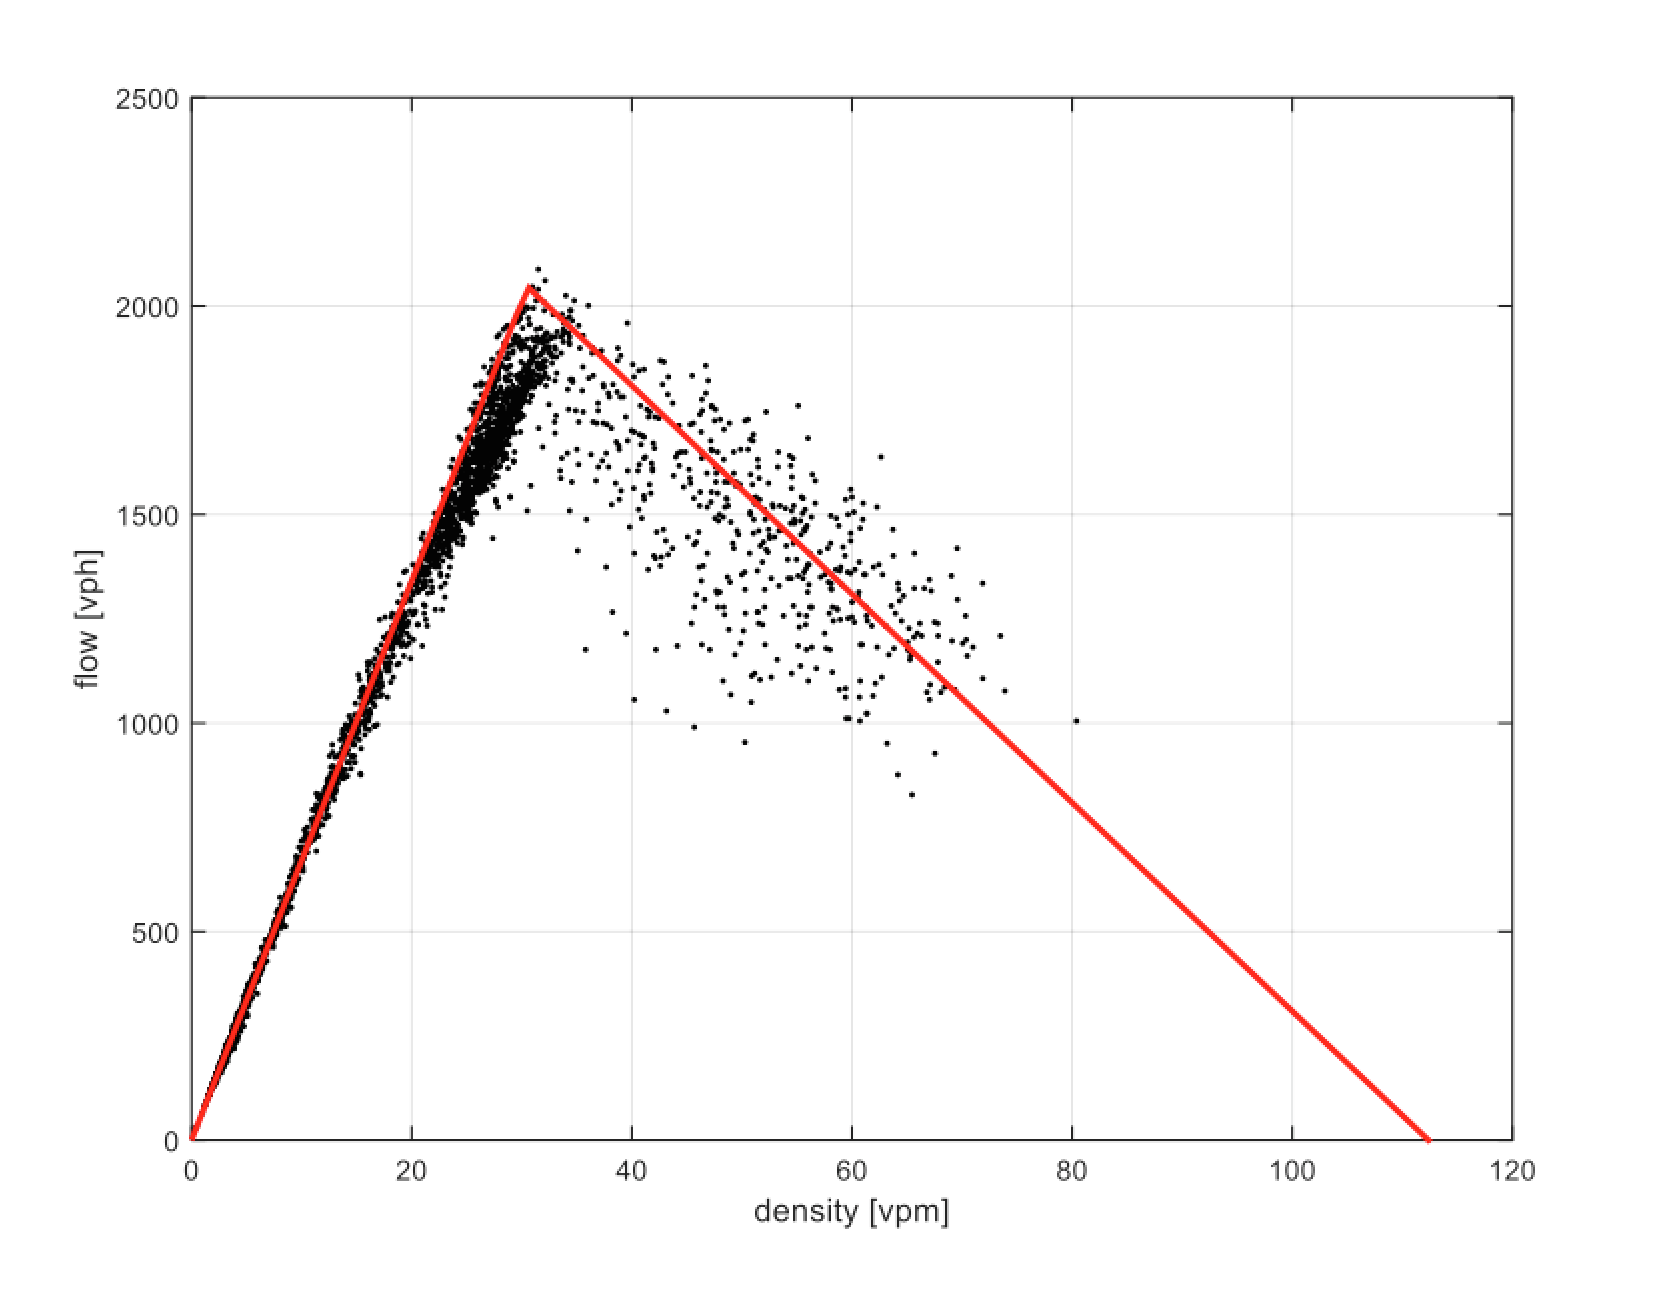
\includegraphics[width=0.8\linewidth]{fd.png}
    \caption{Fundamental Diagram of a Link in I-210 east}
    \label{fig:fd}
\end{figure} 
\subsection{Inspiration}
The aforestated complexities of conventional macroscopic simulators led the authors to exploit the massive amount of traffic data to go beyond piece-wise fundamental diagrams and piece-wise affine dynamics of CTM and perceive a multi-input multi-output function in which time of the day and day of week are taken into account as inputs as well. Clearly, the dynamics and evolution of traffic variables is captured by the recorded data regardless of whether there exists a triangular fundamental diagram dictating flow-density relations for a given link or not, revealing the fact that there is no need for burdensome process of calibration. Moreover, simulation performance and accuracy can perhaps improve; for, extra information such as date and time are provided to the trained multi-layer neural network model \cite{neuralForcast}.  





\section{Data Analysis}
\subsection{PeMS Data} 
PeMS (Performance Measurement System) is a traffic metrics measurement system all over California deployed to obtain loop detector data in real time \cite{PemsPravin}. Freeway PeMS data consists of measurements of vehicular flow, occupancy (fraction of time a vehicle is present on the loop \cite{occupancy}) and speed in time intervals of $5$ minutes. PeMS data is available to users at \url{http://pems.dot.ca.gov/}. In this project, I-210 east (Figure \ref{fig:210}) PeMS data was used as the training and validation data set. 
\begin{figure}[h]
    \centering
    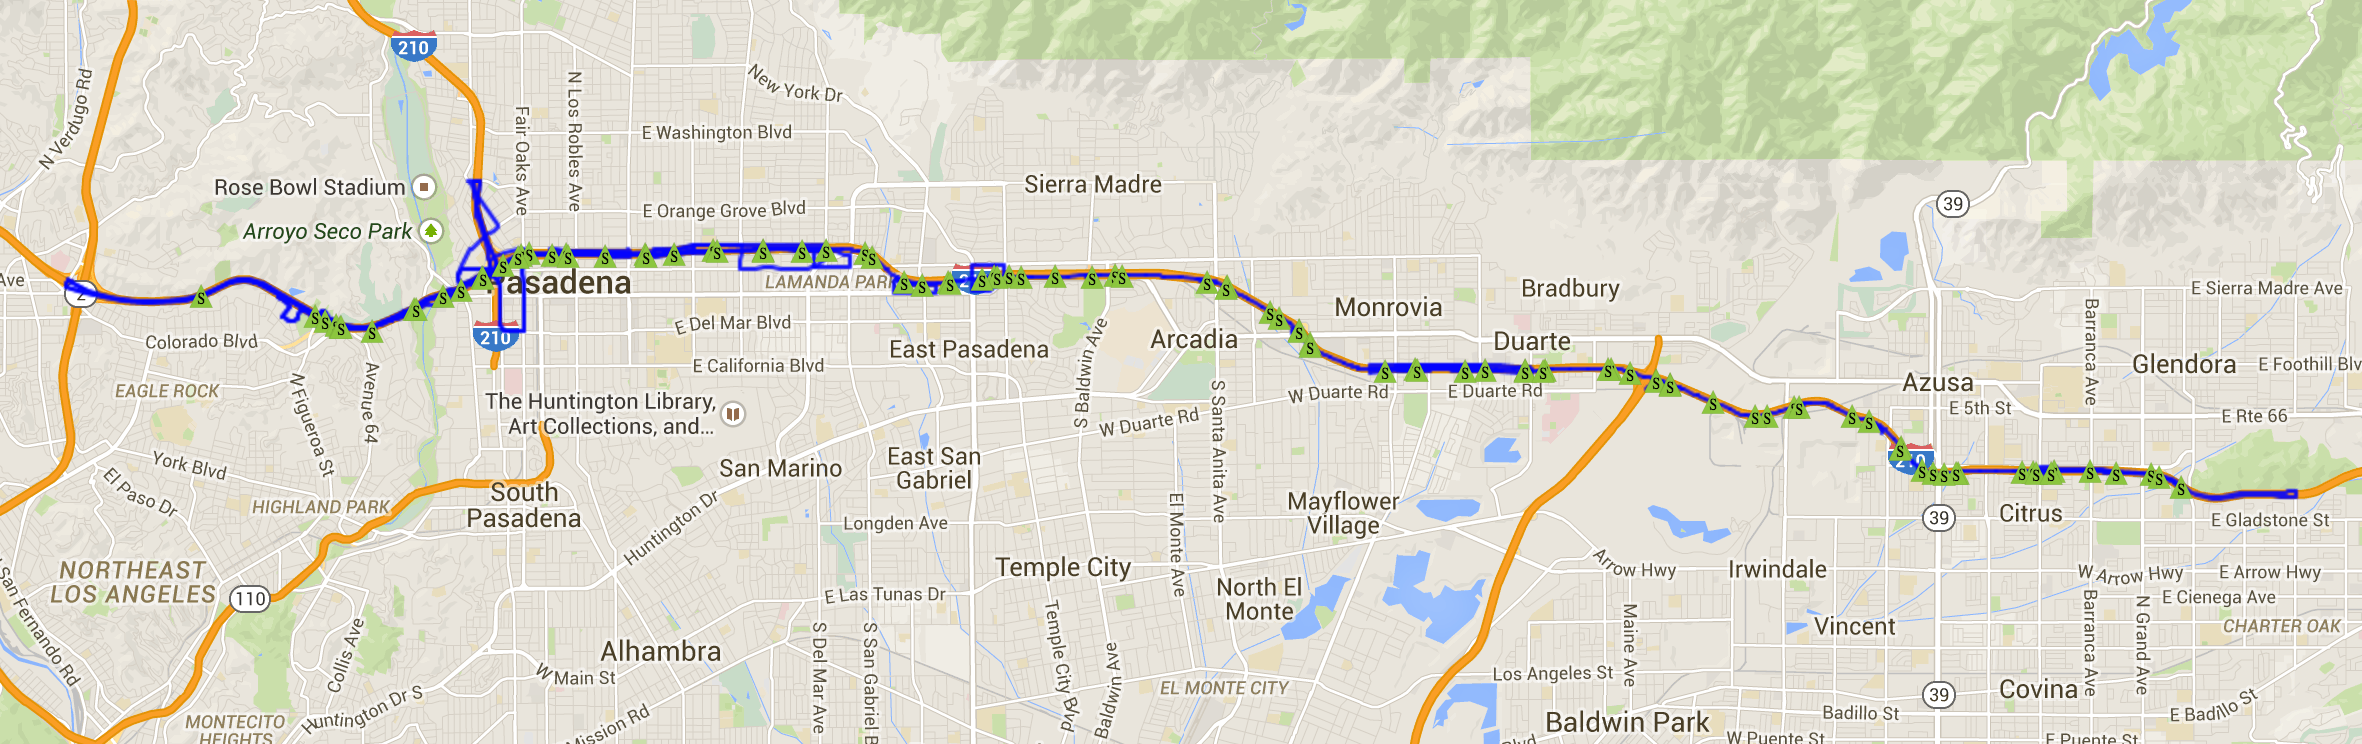
\includegraphics[width=1\linewidth]{210.png}
    \caption{I-210 East Topology}
    \label{fig:210}
\end{figure} 


\subsection{Training Data}

As mentioned previously, since traffic behavior is highly dependent on time of the day and date, our training data consists of flow, occupancy, speed, date and time of day for a single VDS (vehicle detection station) of I-210. Each day is divided into 288 intervals where each time interval lasts $5$ minutes. This data was collected for the last three months of 2014 (October 1\textsuperscript{st} to December 31\textsuperscript{st}).
\subsection{Training Method}
Our main focus of data training was obtaining one-step prediction of traffic behavior; in other words, giving the features of a particular time step of a specific day as the inputs, the outputs should be flow, speed and occupancy of the considered VDS in the next time step. In order to get such a prediction function, a multi-layer neural network was trained on the data, whose characteristics such as number of hidden nodes and number of hidden layers were obtained by cross-validation over a range of node numbers and number of layers.

\subsubsection{Neural Network Layout}

\begin{figure}[t]
	\centering
	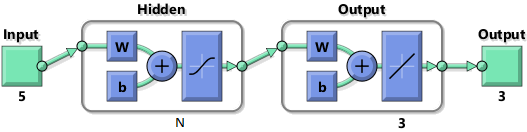
\includegraphics[width=1\linewidth]{./Figures/NN_1}
	\caption{Initial neural-network layout with one hidden and one output layer that have \emph{tanh} and \emph{linear} activation functions respectively }
	\label{fig:nn1}
\end{figure} 

It is known by Universal Approximation Theorem  \cite{universality} that any continuous function on a bounded domain can be approximated by a two-layer neural network with a finite number of hidden nodes. Thereby, the very first step in implementing a NN (deep) learning algorithm is to start with a neural network that has one hidden layer and one output layer as shown in Fig.~\ref{fig:nn1}. 

In such an architecture, there are three crucial design parameters, namely the number of nodes in the hidden layer, the activation functions for the nodes and the cost function that is desired to be minimized when the trained network is applied to test data. In our running example, the number of nodes in the output layer is 3 since the output vector contains the measurements of \emph{flow}, \emph{occupancy} and \emph{speed}. The input vector, here, contains the same signals with one step delay as well as the corresponding time and day number (i.e. a vector in $\mathbb{R}^5$). 

As mentioned above, a design parameter determining structure of the network is number of hidden nodes, denoted by $N$ in Fig.~\ref{fig:nn1}, that should be determined prior to the training process. In order to decide on the ``optimal'' number of hidden nodes, a range of values from $2$ to $80$ was chosen. We considered \emph{tanh} as the activation function for the neurons in the hidden layer, and a pure \emph{linear} function for the output layer nodes (c.f. Fig.~\ref{fig:nn1}). The available data was divided to training, validation and test data sets. These sets, respectively, held 70\%, 15\% and 15\% of the full data set.
Levenberg-Marquardt backpropagation \cite{hagan1994training} since it is often one of the fastest backpropagation algorithm, and it is usually recommended as a first-choice supervised algorithm.
Like the quasi-Newton methods, the Levenberg-Marquardt algorithm was designed to approach second-order training speed without having to compute the Hessian matrix. 
We chose MSE (mean squared error) as the optimization cost function. Validation vectors are used to stop training early if the network performance on the validation vectors fails to improve or remains the same for max-fail epochs in a row. Test vectors are used as a further check that the network is generalizing well, but do not have any effect on training. In MATLAB, training stops when any of these conditions occurs:
\begin{enumerate}
\item The maximum number of epochs (repetitions) is reached.
\item The maximum amount of time is exceeded.
\item Performance is minimized to the goal.
\item The performance gradient falls below min-grad.
\item $\mu$ exceeds $\mu_{\max}$.
\item Validation performance has increased more than max-fail times since the last time it decreased (when using validation).
\end{enumerate}
Training for each set of parameters is performed with different random initializations to avoid being trapped in local minima and the the performance of trained network is shown in Fig~\ref{fig:perf1}. This figure indicates that the best performance is achieved by approximately $50$ nodes in the hidden layer when the activation function is \textit{tanh}.
\begin{figure}[t]
	\centering
	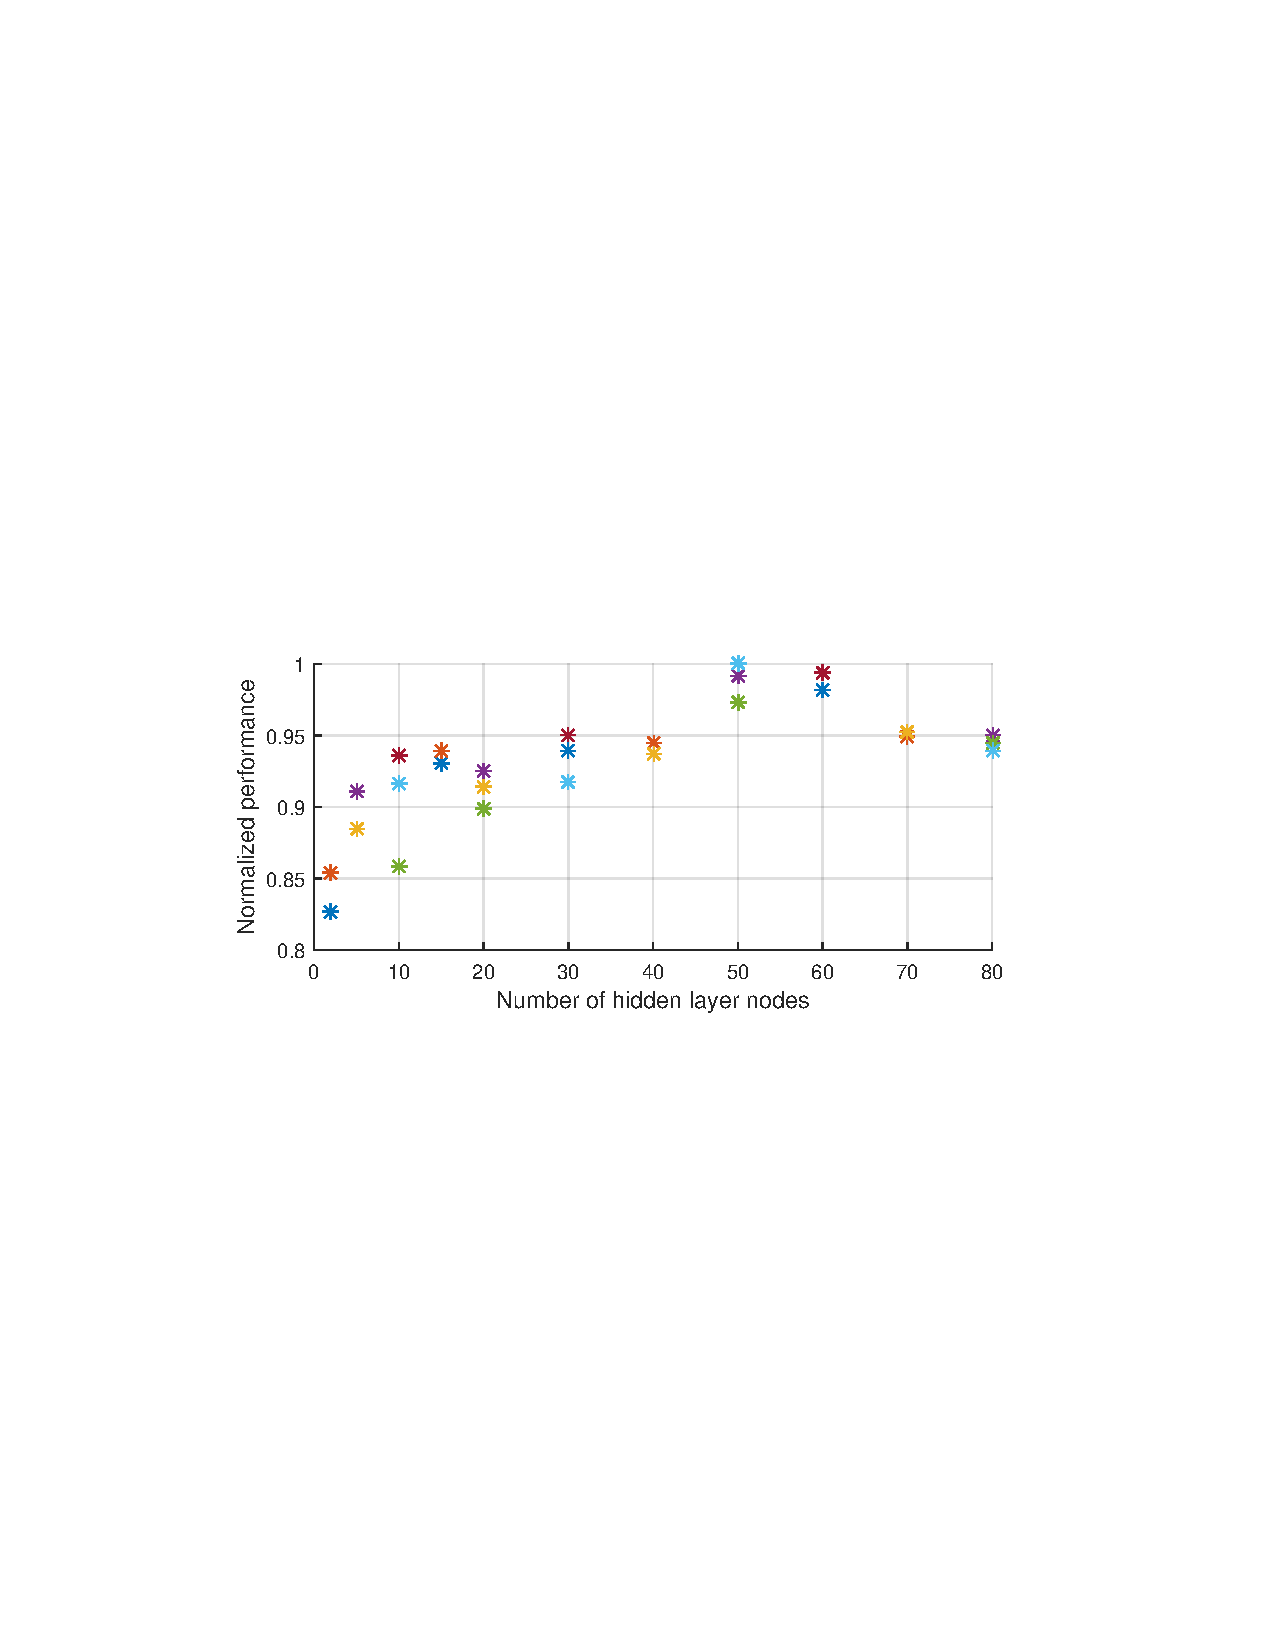
\includegraphics[width=1\linewidth]{./Figures/perf1}
	\caption{ The performance of trained neural network being normalized by the maximum achieved performance versus the number of nodes in the hidden layer when \emph{tanh} and \emph{linear} activation functions are used. }
	\label{fig:perf1}
\end{figure} 

 Different activation functions including radial basis, sigmoid and tangent hyperbolic were examined among which \textit{tanh} performed better by far and chosen as the activation function accordingly.  
The next step is determination of number of layers in the desired network. The question of what is the best of way of configuring a particular number of nodes (in this case $50$) should be addressed. Evidently, best in the optimal sense is obtained by optimizing over the whole set of possible configurations of the network which is practically impossible; hence, performance of several configurations of the network with $50$ nodes is compared (figure \ref{}) where the best performance is obtained by $x$ number of layers where first layer has $x$ number of nodes...

 


\bibliographystyle{plain}
\bibliography{references}

%%%%%%%%%%%%%%%%%%%%%%%%%%%%%%%%%%%%%%%%%%%%%%%%%%%%%%%%%%%%%%%%%%%%%%
\appendix       %%% starting appendix
\section*{Appendix A: Head of First Appendix}
Avoid Appendices if possible.



\end{document}
